\documentclass[12pt]{article}
\usepackage{mathptmx}
\usepackage[utf8]{inputenc}
\usepackage[T1]{fontenc}
\usepackage[left=2.5cm,top=2.5cm,right=2.5cm,bottom=2.5cm,bindingoffset=0.5cm]{geometry}
\usepackage[onehalfspacing]{setspace}
\usepackage{graphicx}
\usepackage[american]{babel}
\usepackage{subcaption} 
\usepackage{morefloats}


\usepackage{csquotes}
\usepackage[style=apa, alldates=year, urldate=short, uniquename=false]{biblatex}
\DeclareLanguageMapping{american}{american-apa}
\usepackage{abstract}

\addbibresource{refs.bib}

\urlstyle{same}

\title{Tactile acuity and visuo-tactile multisensory integration in the context of deafness}
\author{Felix Benjamin Schlüter}
\date{}
%------------------------------------------------------------------------
\begin{document}
%TITLEPAGE-------------------------------------------------------------
\begin{titlepage}
   \begin{center}
       \vspace*{1cm}
%
       \textbf{\huge{Tactile acuity and visuo-tactile multisensory integration in the context of deafness}}\\
% 
       \vspace{0.5cm}
%
       \vspace{1.5cm}
%
\textbf{Felix Benjamin Schlüter*}\\
       \vspace{1.5cm}
       Supervisors:\\
       \vspace{1.5cm}
      \begin{minipage}{0.35\textwidth}
            \centering
            \textbf{Arjan Blokland, PhD}\\
            Head of Department Neuropsychology and Psychopharmacology\\
            Faculty of Psychology  and Neuroscience\\
            Maastricht University,\\
            the Netherlands\\
      \end{minipage}
      \hspace{1.5cm}
      \begin{minipage}{0.35\textwidth}
            \centering
            \textbf{Franco Lepore, PhD}\\
            Director of CERNEC\\
            (Centre de recherche en neuropsychologie et cognition)\\
            Département de psychologie\\
            Université de Montréal,\\
            Canada\\
            \vspace{\baselineskip}
       \end{minipage}
       \vfill
 
       A thesis presented for the degree of\\
       Bachelor of Science
 
       \vspace{0.8cm}
 
       
\includegraphics[width=0.4\textwidth]{UMLogo.png}
 
       *Faculty of Psychology and Neuroscience\\
       Maastricht University,\\
       the Netherlands\\
       May 20, 2019
 
   \end{center}
\end{titlepage}
%-----------------------------------------------------------------
\newpage
\tableofcontents
\newpage
%-----------------------------------------------------------------
\section{Abstract}
Compensatory plasticity due to sensory deficit or loss is thought to be the underlying mechanism of changes in sensory processing. It has previously been investigated whether compensatory plasticity observed in blind and deaf human participants manifests on the behavioral level, however findings are rather inconsistent. Besides focusing on changes in individual sensory modalities, researchers have also investigated changes in multisensory integration. Current findings mainly point to the conclusion that sensory deficit or loss leads to deficits in multisensory integration. The aim of the present study was to add to the understanding of consequences of deafness on tactile acuity and visuo-tactile multisensory integration. One congenitally deaf subject (\textit{n} = 1) and four normal-hearing controls (\textit{n} = 4) performed a vibrotactile frequency discrimination task to assess tactile acuity and a visuo-tactile redundant target paradigm to assess visuo-tactile multisensory integration. The deaf subject in our sample showed levels of tactile acuity and multisensory integration comparable to the levels of normal-hearing controls. Redundancy gains observed for multisensory stimuli in the visuo-tactile redundant target paradigm consistently exceeded race model predictions and were therefore attributed to a coactivation process. 
%
\vspace{1.0cm}\\
\textbf{Keywords}:\textit{ deafness, tactile acuity, vibrotactile frequency discrimination, multisensory integration, visual, tactile, cross-modal plasticity, compensatory plasticity}
%
\section{Introduction}
Every day we are confronted with a multitude of sensory inputs that are processed by our complex human sensory systems. These sensory systems have evolved constantly over time to allow us to make sense of our surroundings. It comes as no surprise, that an extensive  amount of research has been dedicated to understanding the different sensory modalities and how they interact with each other to produce coherent perception. Studies have shown repeatedly that the deficit or loss of one sensory modality can lead to changes in processing in the remaining intact sensory modalities, both in animal models \parencite{lomber_cross-modal_2010, rauschecker_compensatory_1995, schroeder_somatosensory_2001} and in humans \parencite{bavelier_visual_2000,gougoux_pitch_2004, hong_lore_central_1991, levanen_vibration-induced_1998, shiell_enhancement_2014}. 
\par Meaningful insights into these changes mainly stem from research on cross-modal plasticity in blind and deaf individuals using methods ranging from electroencephalography (EEG) and magnetoencephalography (MEG), to positron emission tomography (PET), functional magnetic resonance imaging (fMRI) and transcranial magnetic stimulation (TMS) \parencite[for reviews, see][]{bavelier_deaf_2006,bavelier_cross-modal_2002,merabet_neural_2010,roder_compensatory_2004,voss_adaptation_2010}. The term cross-modal plasticity describes the adaptive re-organization of brain areas that are usually dedicated to one specific sensory modality in the way that those brain areas become innervated by one or more other sensory modalities \parencite{roder_compensatory_2004}. This kind of neuroplasticity is commonly observed in response to sensory deficits or sensory loss as a result of genetic factors, disease or brain damage. It is therefore also referred to as compensatory plasticity \parencite{lazzouni_compensatory_2014, roder_compensatory_2004}. 
%
\par There is evidence that in blind participants the visual cortex can become activated during tactile tasks \parencite{buchel_different_1998,burton_cortical_2004,cohen_functional_1997,sadato_activation_1996} as well as during auditory tasks \parencite{gougoux_functional_2005,kujala_visual_1995,voss_differential_2008}, providing evidence for the occurrence of compensatory plasticity in this population.
Whether compensatory plasticity observed in the blind translates to altered performance on the behavioral level has also been investigated, yet findings are somewhat inconsistent \parencite{merabet_neural_2010, theoret_behavioral_2004, voss_adaptation_2010}. It has previously been reported that blind participants outperform sighted controls on more complex auditory tasks, such as monaural spacial localization of sound \parencite{collignon_cross-modal_2008,gougoux_functional_2005,lessard_early-blind_1998} spacial localization of sound in far-space \parencite{voss_early-_2004}, pitch discrimination \parencite{gougoux_pitch_2004} and speech discrimination \parencite{niemeyer_blind_1981}. On the contrary, no differences between the two groups emerged for more simple auditory acuity tasks \parencite{bross_temporal_1982}. Additionally, researchers have reported superior performance of blind participants as compared to sighted participants in different tactile tasks such as grating orientation discrimination \parencite{boven_tactile_2000,goldreich_tactile_2003,wong_tactile_2011}, haptic shape and angle discrimination \parencite{alary_tactile_2008,norman_blindness_2011} , vibrotactile discrimination \parencite{wan_congenital_2010} and texture discrimination \parencite{alary_tactile_2009}. Again, other studies reported no superior tactile performance of blind participants, or only for specific tasks \parencite{alary_tactile_2009,grant_tactile_2000,papagno_deaf_2016}.
%-----------------------------------------------------------------------------
\par Comparable to the blind population, compensatory plasticity as evidenced by activation of the auditory cortex by non-auditory inputs has been reported in deaf participants \parencite[for reviews, see][]{heimler_revisiting_2014, merabet_neural_2010, voss_adaptation_2010}. Activation of the auditory cortex of deaf participants has been reported during visual tasks such as viewing sign language \parencite{nishimura_sign_1999,petitto_speech-like_2000} as well as in response to other kinds of visual stimuli \parencite{finney_visual_2003,karns_altered_2012,sadato_cross-modal_2005}. In addition, auditory cortex activity in deaf participants has been reported during tactile tasks, yet evidence is scarcer as compared to the visual modality \parencite{auer_vibrotactile_2007,levanen_vibration-induced_1998,merabet_neural_2010,schurmann_touch_2006}. Using MEG, Levänen, Jousmäki and Hari (1989) observed activation in auditory cortical regions in response to vibratory tactile stimulation to the palm and finger of congenitally deaf adults. Similarly, but based on fMRI,  Auer, Bernstein, Sungkarat and Sing (2007) reported activity of auditory cortical regions in deaf participants in response to vibratory tactile stimuli delivered to the hand. 
\par In line with research efforts in the blind population, it has also been investigated whether the compensatory plasticity observed in deaf participants manifests on the behavioral level \parencite{heimler_response_2014,heimler_revisiting_2014}. Concerning visual processing, behavioral studies have shown enhanced performance of deaf participants compared to normal-hearing participants, for example in the attentional processing of the peripheral visual field \parencite{proksch_changes_2002} and the discrimination of the direction of visual motion \parencite{hauthal_visual_2013,shiell_enhancement_2014}. In contrast to this, other behavioral studies have failed to show enhanced performance of deaf participants in visual tasks \parencite{bavelier_deaf_2006,brozinsky_motion_2004,hauthal_visual_2013}. 
%---------------------------------------------------------------------------------
\par Evidence for changes in performance of deaf participants in tactile tasks is relatively scarce and inconsistent \parencite{heimler_multisensory_2017,papagno_deaf_2016}. Compared to normal-hearing participants, some studies have shown deaf participants to have lower temporal processing abilities for tactile stimuli \parencite{heming_sensory_2005}, lower ability to discriminate the temporal duration of tactile stimuli \parencite{bolognini_hearing_2011} and less tactile sensitivity as measured by grating orientation discrimination and detection thresholds for vibratory tactile stimuli \parencite{frenzel_genetic_2012, moshourab_congenital_2017}. In contrast to these findings, an early study by Schiff and Dytell (1972) has shown deaf children and adolescents to have enhanced tactile sensitivity as evidenced by lower thresholds for vibratory tactile stimuli and lower thresholds for two-point discrimination compared to a normal-hearing control group. Furthermore, Levänen and Hamdorf (2001) reported an advantage of deaf participants to detect infrequent suprathreshold vibratory tactile stimuli presented within the sequence of a fixed vibratory tactile reference stimulus, compared to normal-hearing participants. Additionally, the authors reported a trend of lower thresholds for deaf participants compared to normal-hearing controls in the discrimination of frequencies of vibratory tactile stimuli which, however, did not reach significance. Another study by van Dijk, Kappers and Postma (2013) showed that deaf participants outperformed hearing signers and normal-hearing controls in an haptic spatial processing task, yet these results point more towards the conclusion of enhanced visuospatial processing in the deaf, rather than enhanced tactile processing.
%------------------------------------------------------------------
\par It is important to note that most of the evidence of enhanced tactile performance in deaf participants compared to normal-hearing controls stems from studies using vibratory tactile stimuli \parencite{levanen_feeling_2001,schiff_deaf_1972}. In general, it appears that humans are responsive to sinusoidal vibrations of frequencies between 25 Hz and 700 Hz with a spectrum of optimal sensitivity around 250 Hz to 300 Hz \parencite{perez_two-point_2000, verrillo_vibrotactile_1966}. Of the four types of cutaneous mechanoreceptors and their corresponding cutaneous mechanoreceptive afferent neurons in the human skin, the rapidly adapting (RA) afferents which originate in Meissner corpuscles and the Pacinian (PC) afferents which originate in Pacinian corpuscles have been shown to be responsible for the perception of vibrations \parencite{johnson_tactile_2000,johnson_roles_2001}. 
%
\par RA afferents originating in Meissner corpuscles have been shown to be responsible for the detection and discrimination of low frequency vibrations, being most sensitive for vibrations between 40 Hz and 60 Hz \parencite{lamotte_capacities_1975,mountcastle_detection_1972,talbot_sense_1968}. PC afferents originating in Pacinian corpuscles show a rather poor spatial resolution \parencite{phillips_tactile_1981}, but they have been shown to be highly sensitive to vibrations of higher frequencies \parencite{lindblom_discharge_1966,mountcastle_detection_1972,sato_response_1961}. The population of PC afferents produces a robust neural representation of high frequency stimuli which are transmitted to the glabrous skin through objects that are held in hand \parencite{brisben_detection_1999, hunt_nature_1961, johnson_roles_2001}.
%---------------------------------------------------------------------------------------
\par Information of one sensory modality is rarely processed in isolation. Indeed, most of the time we are presented with sensory information from multiple sensory modalities for the same occurring event (e.g. a mobile phone that rings and vibrates simultaneously to indicate an incoming call or message). The process of integrating inputs of multiple sensory modalities (e.g. auditory, tactile and visual) to modulate perception and behavior is referred to as multisensory integration \parencite{calvert_handbook_2004, ernst_merging_2004,stein_merging_1993}. 
%
\par Illusions that arise due to the interplay between two sensory modalities such as the the “parchment skin illusion” \parencite{jousmaki_parchment-skin_1998} or the “double-flash illusion” \parencite{lange_perception_2011, shams_illusions:_2000, violentyev_touch-induced_2005} nicely illustrate the important role of multisensory integration in human perception. The parchment skin illusion is a well-researched effect that is based on the integration of visual and tactile information. In a classic study, participants were instructed to rate the subjectively perceived moistness or dryness while rubbing their palms together. The rubbing sound that the participants produced was recorded, manipulated and then fed back to them via headphones. By manipulating the amplitude of sound components above 2000 Hz the researchers could alter the perceived moistness/dryness to the point, where some participants even reported the sensation having a piece of parchment paper between their palms \parencite{jousmaki_parchment-skin_1998}. The double-flash illusion is an effect which has originally been demonstrated based on the integration of visual and auditory information. When a single visual stimulus (e.g. a white disk on black background) is presented very briefly (flashed) while being accompanied by multiple auditory beeps, participants report perceiving multiple flashes of the visual stimulus instead of one \parencite{shams_illusions:_2000}. Besides this sound-induced flash illusion, researchers have  also successfully demonstrated a touch-induced flash illusion yielding a similar effect based on the integration of tactile and visual information \parencite{lange_perception_2011,violentyev_touch-induced_2005}. 
%
\par A brain area that has been the focus of research in animals investigating the underlying neural mechanisms of multisensory integration is the superior culliculus (SC). The SC is located in the mammalian midbrain and has been shown to be involved in visual perception and attention as well as in the control of head and eye movements \parencite{sprague_role_1965}. This brain area is of special interest to researchers in the domain of multisensory integration as it contains multisensory neurons in its deeper layers (layers IV-VII) which receive inputs from multiple sensory modalities (e.g. auditory, visual and tactile)\parencite{stein_merging_1993,wallace_converging_1993}. Furthermore, the direct involvement of the SC in behavioral aspects of visual attention and perception such as detection, orientation and localization make it a perfect model for studying the neural mechanisms of multisensory integration, as neurophysiological observations can be directly compared to overt behaviors \parencite{bell_crossmodal_2005,burnett_superior_2004,jiang_two_2002,stein_behavioral_1989}. 
%
\par Key findings from this line of research include a number of general rules or principles which seem to govern the process of multisensory integration \parencite[for review, see][]{meredith_interactions_1983,stein_merging_1993}. The “spatial principle” states that multisensory stimuli (stimuli from two or more sensory modalities) more likely lead to multisensory enhancement (meaning a greater response compared to the response induced by unisensory stimuli) if they originate from an approximately similar location in space and thereby fall into overlapping receptive fields of the multisensory neuron \parencite{kadunce_influence_2001, wallace_representation_1996}. If multisensory stimuli originate from different locations in space, this has been shown to elicit either no multisensory enhancement or even lead to response depression (meaning a response smaller than the response elicited by a unisensory stimulus alone) \parencite{meredith_spatial_1996,wallace_representation_1996}. Following a similar logic, the “temporal principle” states that multisensory stimuli lead to greater multisensory enhancement if the combined unisensory stimuli are presented approximately at the same time \parencite{meredith_determinants_1987,recanzone_auditory_2003,wallace_representation_1996}. Lastly, the “principle of inverse effectiveness” states that multisensory enhancement is inversely related to the effectiveness of the individual unisensory stimuli which are combined into a multisensory stimulus. This means that if two, individually highly salient unisensory stimuli are combined, the resulting multisensory enhancement is weaker, compared to the combination of two less salient stimuli  \parencite{alex_meredith_spatial_1986,perrault_superior_2005,wallace_representation_1996}. 
%
\par For the purpose of the present study, we will focus on the evidence of multisensory integration coming from behavioural studies, especially those investigating reaction times of human participants. An early finding of psychophysical studies of human participants is that presenting a combination of two (or more) stimuli of different modalities leads to shorter reaction time compared to when only unimodal stimuli are presented \parencite{hershenson_reaction_1962,todd_reaction_1912}. This early observation has become known as the “redundant signals effect” or “redundant target effect” \parencite{kinchla_detecting_1974,miller_divided_1982,miller_timecourse_1986} and has been replicated multiple times since then \parencite{diederich_bimodal_2004,hughes_visual-auditory_1994,schroger_speeded_1998}. Two main classes of models have been proposed to account for the shortened RT for multisensory stimuli compared to unisensory stimuli, also referred to as “redundancy gain” (RG) or “multisensory gain” \parencite{miller_divided_1982,miller_timecourse_1986,ridgway_redundant_2008,dykes_investigation_1978}. 
%
\par The first class, which has become known as “separate activation models” or “race models”, proposes that a multisensory stimulus produces a parallel but separate activation of the sensory channels belonging to the different sensory modalities that have been combined. Following this model, a response is initiated by the sensory channel which is the first to reach a level of activation, sufficient to trigger a response \parencite{calvert_handbook_2004, miller_divided_1982,miller_timecourse_1986,raab_division_1962}. If we assume (1) a statistical variability in the processing time of the different sensory channels and (2) that the distributions of the processing times of the different sensory channels overlap, race models predict shorter reaction times for multisensory compared to unisensory stimuli due to the fact that the average processing time of the fastest sensory channel is smaller than the average processing time of each single sensory channel. This effect is generally known as “statistical facilitation” or “probability summation” \parencite{miller_divided_1982,raab_division_1962}. 
%
\par The second class of models is referred to as “coactivation models” and proposes that instead of separate activation, the activation of different sensory channels is combined in some stage of processing to collectively trigger a response \parencite{miller_divided_1982,miller_timecourse_1986}. Evidence for coactivation models mainly stems from the observation that redundancy gains for multisensory stimuli often exceed the prediction of race models, meaning that the difference in RT to multisensory stimuli compared to unisensory stimuli is often too high to be explained by race models (i.e. statistical facilitation alone) \parencite{miller_divided_1982,miller_timecourse_1986}. Miller (1982) introduced a distribution inequality test in which he tested for the violation of assumptions of race models (“race model inequality”) by comparing the distribution functions of reaction times from multisensory stimulation and unisensory stimulation, a test that has been refined and applied in many subsequent behavioral studies of multisensory integration \parencite{colonius_race_2006, diederich_probability_1992,forster_redundant_2002,giard_auditory-visual_1999,girard_multisensory_2011, gondan_testing_2008}.
%------------------------------------------------------------------------------------------
\par Given the fact that changes in sensory processing as evidenced by compensatory plasticity and behavioral changes have been observed in the remaining intact senses following sensory loss or deficit, researchers have also started to investigate the effects of sensory loss or deficit on multisensory integration \parencite{champoux_early-_2011,collignon_further_2009,hauthal_visuo-tactile_2015,hotting_hearing_2004,karns_altered_2012,landry_temporary_2013,nava_audio-tactile_2014,occelli_audiotactile_2012,peter_sensory_2019}. For example, Champoux and colleagoues (2011) showed that blind participants were not susceptible to the parchment-skin illusion, indicating deficits in audiotactile integration compared to sighted controls. Another study by Occelli, Bruns, Zampini and Röder (2012) demonstrated that blind participants show a reduced ventriloquism effect compared to sighted controls. This effect arises when the localization of sound is biased by the simultaneous presentation of visual stimuli. A reduced ventriloquism effect in blind participants therefore also indicates a deficit in audiotactile integration \parencite{occelli_audiotactile_2012}. Hauthal and colleagues (2015) used a visuo-tactile redundant target paradigm together with EEG recording to investigate differences in visuo-tactile multisensory integration between congenitally deaf and normal-hearing participants. Even though they found no difference in the detection of unisensory visual and unisensory tactile stimuli between the deaf and normal hearing group, they did find that deaf participants profited significantly less from multisensory integration in terms of redundancy gain (i.e. reduced reaction time) in response to multisensory stimuli compared to normal-hearing participants \parencite{hauthal_visuo-tactile_2015}. Furthermore, researchers found that previously deaf participants whose hearing was restored to normal at a later point in their life by means of a cochlear implant are significantly less susceptible to an audio-tactile double flash illusion compared to normal-hearing participants \parencite{landry_temporary_2013}. Taken together, these findings support the conclusion that the process of multisensory integration can be altered or disrupted by the deficit or loss of one sensory modality (e.g. hearing or vision).
%-----------------------------------------------------------------------------------------
\par The present study intends to add to the understanding of differences in tactile acuity and multisensory integration between congenitally deaf and normal-hearing individuals. For this purpose, the performance on a vibrotactile frequency discrimination task and a visuo-tactile redundant target paradigm was compared between a congenitally deaf participant and a control group of normal-hearing participants. The vibrotactile frequency discrimination task we used was a a two-interval forced-choice (2IFC) paradigm mainly adapted from Alary and colleagues (2009) with minor changes concerning the frequencies of the vibrotactile stimuli and the total number of trials that were administered. Reaction times were recorded for each participant. Based on previous research by Levänen and Hamdorf (2001) and Schiff and Dytell (1972), we hypothesized that the deaf participant would show enhanced tactile acuity compared to normal-hearing participants which would result in shorter reaction times on the vibrotactile frequency discrimination task, especially for small  differences in frequency (Hz). The visuo-tactile redundant target paradigm was mainly adapted from Girard, Collingnon and Lepore (2011) but included only a simple reaction time condition. Reaction times were recorded and redundant target effects were examined for the deaf participant and normal-hearing participants to determine whether average reaction times were faster for multisensory compared to unisensory stimuli. Redundancy gain was then compared between groups. Furthermore, Miller’s (1982) race model inequality was assessed using RMITest software by Ulrich, Miller and Schröter (2007) to determine whether the observed redundancy gain can be explained by a coactivation process. Based on previous research by Hauthal, Debener, Rach, Sandmann and Thorne (2015), we hypothesized that deaf participants would show less redundancy gain compared to normal-hearing participants, indicating that visuo-tactile multisensory integration is disrupted due to sensory deficit.

\section{Methods}
%--------------------------------------------------------------------------------------
\subsection{Participants}
One congenitally deaf participant showing profound bilateral hearing loss (\textit{n} = 1) and four normal hearing participants (\textit{n} = 4) participated in the present study. The deaf participant was recruited by personal acquaintance. Normal-hearing participants were recruited using written public announcements on blackboards on the campus of the Université de Montréal and on social media platforms. All participants presented normal levels of tactile sensation and normal or corrected vision. Participants with a history of neurological or psychiatric disorders were excluded from the study. The study was approved by the local ethics committee of the Université de Montréal and all participants gave their written consent before participating in the study. Furthermore, participants were financially compensated for their participation.
%---------------------------------------------------------------------------------------
\subsection{Tasks and Procedures}
All participants performed a computerized vibrotactile frequency discrimination task to investigate tactile acuity to vibratory stimuli and a computerized visuo-tactile redundant target paradigm to investigate visuo-tactile multisensory integration. The order of administration of the two tasks was counterbalanced between participants.
%----------------------------------------------------------------------------------------
\subsubsection{Vibrotactile frequency discrimination task}
The procedure for the vibrotactile frequency discrimination was mainly based on the protocol used by Alary et al. (2009). However, the standard vibrotactile frequency was adjusted based on previous studies including deaf participants \parencite{auer_vibrotactile_2007} and a greater total number of trials was administered. Participants were seated in a sound-attenuated room in front of a computer screen and placed their dominant hand on top of the acrylic glass box of the custom-designed non-magnetic vibrotactile stimulation device which was placed on a table in front of them. The participants hand was placed in a way that the distal phalanx of the index finger made contact with a wooden contact piece through a 9 mm x 25 mm  window on top of the acrylic glass box \parencite[see][]{alary_tactile_2009}. The participants non-dominant hand was placed on a numeric keypad on which the participant indicated his response on each trial by pressing one of two keys assigned to the two possible responses. During the whole experiment, participants were instructed to fixate a fixation cross presented on the computer screen in front of them. Furthermore, to prevent confounding due to auditory cues, participants wore ear plugs and noise-cancelling headphones and white noise was played through loudspeakers inside the sound-attenuated room where the experiment took place.
%-----------------------------------------------------------------------------------
\begin{figure*}[t!]
    \centering
    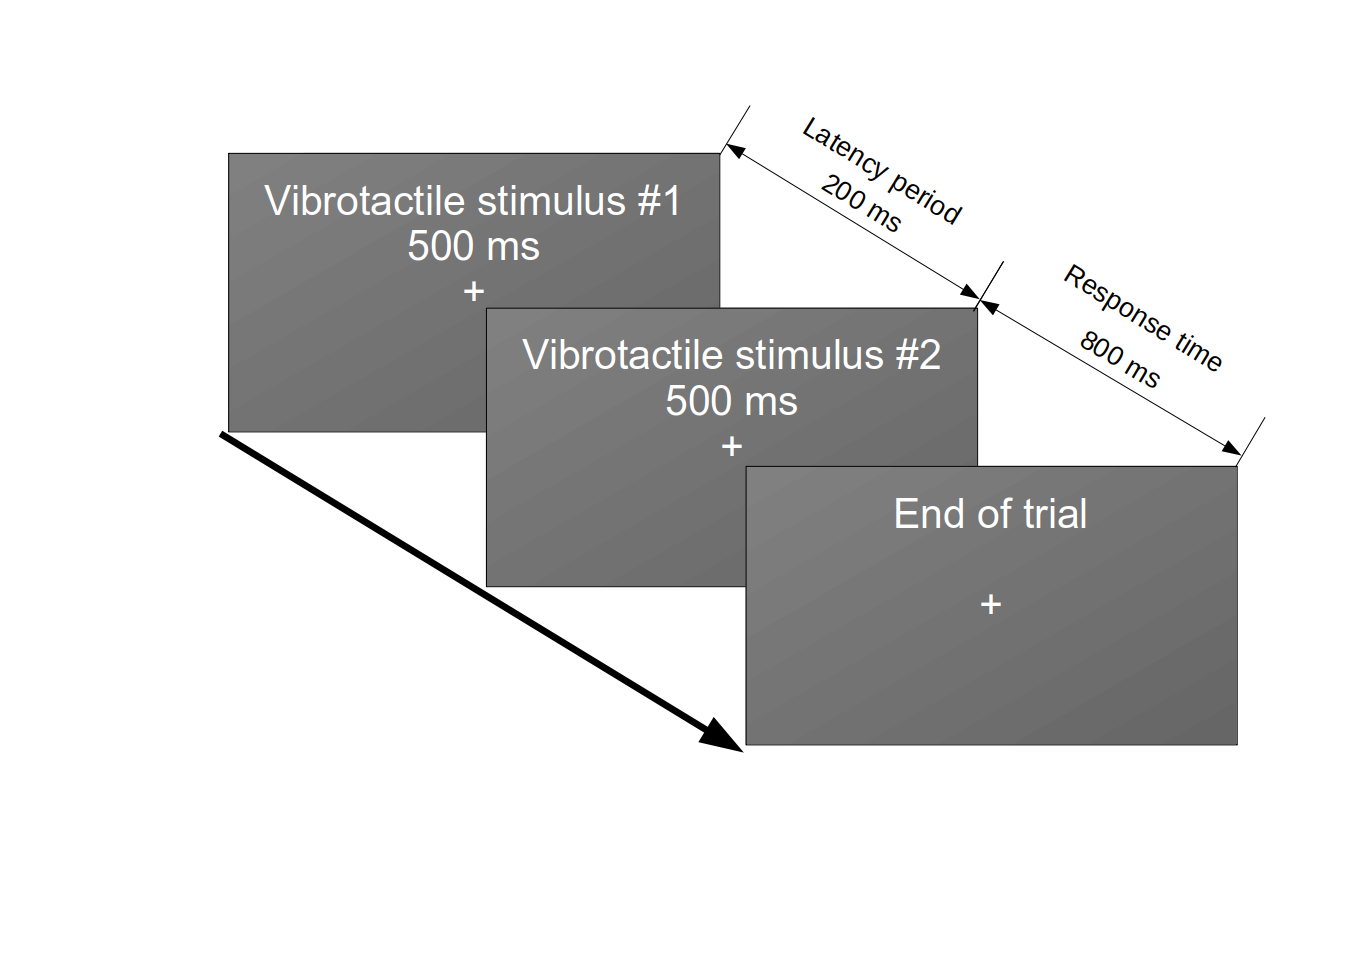
\includegraphics[width=0.8\textwidth]{VTFD_overview.png}
    \caption{\textit{\footnotesize{Schematic overview of a trial in the vibrotactile frequency discrimination task.}}}
    \label{fig:VTFD}
\end{figure*}
%
\par In a computerized two-interval forced choice (2IFC) paradigm two vibrotactile stimuli of a duration of 500 ms each were administered to participants separated by a 200 ms latency period (see Figure 1). One of the intervals contained the standard vibrotactile stimulus of 125 Hz \parencite[adapted from][]{auer_vibrotactile_2007}. The other interval contained either the standard 125 Hz stimulus or a modification of the standard stimulus which could have an intensity between 130 Hz and 175 Hz with increments being made in steps of 5 Hz, resulting in a total of 10 possible increments. Following the presentation of the second stimulus, participants had 800 ms to indicate whether they perceived the two presented stimuli to be of (1) the same or (2) differing frequencies by using the numeric keypad. 
%
\par A number of 60 trials per combination of standard stimulus and modified stimulus was administered. In 30 out of these 60 trials the standard 125 Hz stimulus was presented in the first interval and the modified stimulus was presented in the second interval while in the other 30 trials the modified stimulus was presented first, followed by the standard 125 Hz stimulus. Together with the combination in which both intervals contained the standard125 Hz stimulus, this results in  a total of 660 trials. The total of 660 trials was spread over 6 blocks in which stimulus combinations were presented in a randomized order. Participants were instructed to respond as fast and accurately as possible and reaction times were recorded. Stimulus presentation and the recording of responses and reaction times was controlled using Presentation software (Neurobehavioral Systems Inc.).
%--------------------------------------------------------------------------------------------------
%
\begin{figure*}[t!]
    \centering
    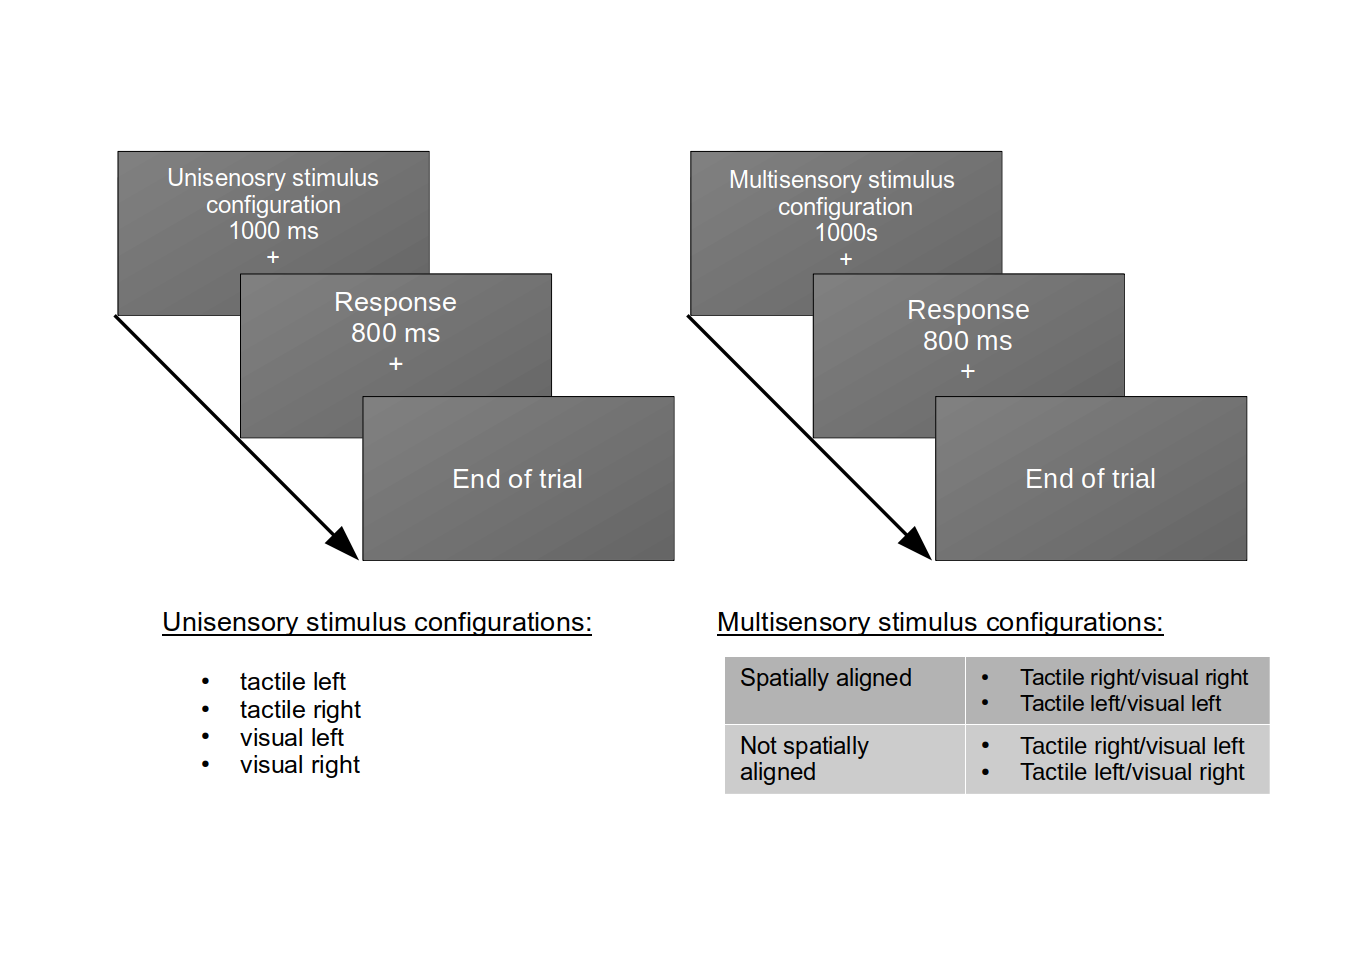
\includegraphics[width=0.9\textwidth]{VVTMI_overview.png}
    \caption{\textit{\footnotesize{Schematic overview of trials in the visuo-tactile redundant target paradigm. \textbf{Left}: trial presenting a unisensory stimulus configuration. \textbf{Right}: trial presenting a multisensory stimulus configuration. \textbf{Bottom}: possible unisensory and multisensory stimulus configurations.}}}
    \label{fig:VVTMI}
\end{figure*}
%
\subsubsection{Visuo-tactile redundant target paradigm}
The procedure of the visuo-tactile redundant target paradigm was mainly adapted from Girard, Collingnon and Lepore (2011) but included only a simple reaction time condition. Participants were seated in front of a table and a computer screen in a dark, sound-attenuated room. Two of the custom designed non-magnetic vibrotactile stimulation devices that were also used in the vibrotactile frequency discrimination task were used to deliver tactile stimulation. The two stimulation devices were placed on the left and right side of the table in front of the participant. For this part of the experiment, participants placed their left hand on top of the vibrotactile stimulation device to their left and their right hand on top of the vibrotactile stimulation device to their right. 
Again, the participants hands were placed in a way that the distal phalanx of the index finger of each hand made contact with a wooden contact piece through the 9 mm x 25 mm  window on top of the acrylic glass box \parencite[see][]{alary_tactile_2009}. %
\par Tactile stimuli consisted of sinusoidal vibrations with a frequency of 125 Hz \parencite[adapted from][]{auer_vibrotactile_2007} delivered to the left or right hand for a duration of one second. Visual stimuli were presented via the computer screen and consisted of a white circle presented on a black background either to the right or the left side of a central fixation cross for one second .Visual stimuli were presented far enough to the left or right visual field to ensure that they activated the contralateral visual cortex only \parencite[see][]{girard_multisensory_2011}. Tactile stimuli and visual stimuli could be presented either in a unisensory configuration (only tactile or only visual) or in a multisensory manner (tactile and visual combined). When presented in a multisensory configuration, the stimuli could either be presented spatially aligned (e.g. tactile right/visual right) or not spatially aligned (e.g. tactile right/ visual left). This results in a total of eight possible stimulus configurations: four unisensory configurations and four multisensory configurations (see Figure 2). Participants were instructed to react as fast and accurately as possible to any kind of stimulation, irrespective of spatial alignment. Participants indicated their answer by pressing a key on a numeric keypad. The numeric keypad was positioned on the side of the participants dominant hand next to the vibrotactile stimulation device and participants used their thumb to press the key. 
%
\par One trial included the presentation of the stimulus for one second after which participants had 800 ms to indicate their answer on the numeric keypad followed by a latency period of 500 ms before the next trial started.  The eight stimulus configurations were presented in 120 trials each, resulting in an overall total of 960 trials. This total number of trials was divided into 8 blocks including 15 trials per stimulus configuration, resulting in a total of 120 trials per block. To prevent confounding due to auditory cues, participants wore ear plugs and noise-canceling headphones and white noise was played through loudspeakers inside the sound-attenuated room where the experiment took place. Stimulus presentation and the recording of reaction times was controlled using Presentation software (Neurobehavioral Systems Inc.).
%--------------------------------------------------------------------------------------------
\subsection{Data analysis}
%--------------------------------------------------------------------------------------------
Due to insufficient performance in terms of accuracy (below chance level for the majority of stimulus combinations in the vibrotactile frequency task) participant four was be removed from the analysis, resulting in a total of one congenitally deaf participant (\textit{n} = 1) and three normal-hearing participants (\textit{n} = 3). Given the very low total sample size (\textit{N} = 4), it was not possible to make inferences about differences on the population level. Instead the analysis is limited to the individual trials and the effects on the sample level only.
%--------------------------------------------------------------------------------------------
\subsubsection{Vibrotactile frequency discrimination task}
To investigate differences in tactile acuity, the reaction times of the deaf participant and normal-hearing participants obtained in the vibrotactile frequency discrimination task were compared for a selection of three pairs of stimulus combinations using analysis of variance (ANOVA) (GLM Univariate, IBM SPSS Statistics for Windows, Version 25.0). To account for the increase in probability of making a Type I error due to multiple comparisons, the \textit{alpha} significance level was adjusted to 0.0167 (0,05/3). 
%
\par First, differences between participants in terms of reaction times were compared between the stimulus combination of the 125 Hz and 125 Hz stimulus and the stimulus combination of the 125 Hz and 130 Hz stimulus to investigate differences in reaction time for no difference in frequency compared to a small 5 Hz difference. As we intended to investigate whether the effect of the stimulus combination differed between the deaf and the normal hearing participants, an interaction effect between stimulus combination and participants was of particular interest. In order to be able to test this interaction effect, the model for this analysis was a 2 x 4 x 469 mixed model, including the difference in frequency between stimuli as the first fixed factor with two levels (0 Hz difference and 5 Hz difference), participants as the second random factor with four levels and trials as the third fixed factor with 469 levels representing the number of valid trials. The model was tested using a three-way within-subjects ANOVA (GLM Univariate, IBM SPSS Statistics for Windows, Version 25.0). A Helmert contrast was applied to the random factor participant (deaf participant = 1) to compare between the deaf participant and all normal-hearing participants. 
%
\par A similar three-way within-subjects ANOVA (GLM Univariate, IBM SPSS Statistics for Windows, Version 25.0) was conducted, this time comparing between the stimulus combination of 125 Hz and 130 Hz and the stimulus combination of 125 Hz and 175 Hz to investigate differences in reaction time for a small 5 Hz difference compared to a large 50 Hz difference. Again, the model was a 2 x 4 x 472 mixed model, including the difference in frequency between stimuli as the first fixed factor with two levels (5 Hz difference and 50 Hz difference), participants the second random factor with four levels and trials as the third fixed factor with 472 levels representing the number of valid trials . Similar to the analysis before, a Helmert contrast was applied to the random factor participant (deaf participant = 1) to compare between the deaf participant and all normal-hearing participants. 
%
\par Lastly, another three-way within-subjects ANOVA (GLM Univariate, IBM SPSS Statistics for Windows, Version 25.0) was conducted, comparing between the stimulus combination of 125 Hz and 170 Hz (45 Hz difference) and the stimulus combination of 125 Hz and 175 Hz (50 Hz difference) to investigate differences in reaction time between a large 45 Hz difference and the maximum 50 Hz difference. Consistent with the analyses  before, the model was a 2 x 4 x 474 mixed model, including the difference in frequency between stimuli as the first fixed factor with two levels (45 Hz difference and 50 Hz difference), participants the second random factor with four levels and trials as the third fixed factor with 474 levels representing the number of valid trials. A Helmert contrast was applied to the random factor participants (deaf participant = 1) to compare between the deaf participant and all other participants.
%--------------------------------------------------------------------------------------------
\subsubsection{Visuo-tactile redundant target paradigm}
To investigate the effect of different stimulus configurations (multisensory vs. unisensory and spatially aligned vs. non-spatailly aligned) on multisensory integration and the differences between the deaf participant and normal-hearing participants, the reaction times obtained in the visuo-tactile redundant target paradigm were analyzed using analysis of variance (ANOVA) (GLM Univariate, IBM SPSS Statistics for Windows, Version 25.0). To account for the increase in probability of making a Type I error due to multiple comparisons, the \textit{alpha} significance level was adjusted to 0.025 (0,05/2). 
%
\par First, differences in reaction time for multisensory stimulus configurations and unisensory stimulus configurations were compared between the deaf and normal hearing participants. As the intention again was to investigate whether the effect of the stimulus configuration differed between the deaf participant and the normal hearing participants, an interaction effect between stimulus combination and participants was of particular interest. In order to be able to test this interaction effect, the model for this analysis was a 2 x 4 x 3840 mixed model, including stimulus configuration as the first fixed factor with two levels (unisensory and multisensory), participants as the second random factor with four levels and trials as the third fixed factor with 3840 levels representing the number of valid trials. The model was analyzed using a three-way within-subjects ANOVA (GLM Univariate, IBM SPSS Statistics for Windows, Version 25.0) and a Helmert contrast was applied to the random factor participant (deaf participant = 1) to compare between the deaf participant and all normal-hearing participants. 
%
\par Secondly, differences in reaction time between spatially aligned multisensory stimulus configurations (visual left/tactile left, visual right/tactile right) and non-spatially aligned multisensory stimulus configurations (visual right/tactile left, visual left/tactile right) were compared between the deaf and normal hearing participants. The model for this analysis was a 2 x 4 x 3840 mixed model, including stimulus configuration as the first fixed factor with two levels (spatially aligned and not spatially aligned), participants as the second random factor with four levels and trials as the third fixed factor with 3840 levels representing the number of valid trials. The model was analyzed using a three-way within-subjects ANOVA (GLM Univariate, IBM SPSS Statistics for Windows, Version 25.0) and a Helmert contrast was applied to the random factor participant (deaf participant = 1) to compare between the deaf participant and all normal-hearing participants.
%-------------------------------------------------------------------------------------------
\par The analysis of race model inequality was similar to the analysis conducted by Girard, Collingnon and Lepore (2011). In general, a violation of the race model was tested by comparing reaction times obtained in trials of multisensory stimulus configurations to reaction times obtained in trials of unisensory stimulus configurations. It was then determined whether the redundancy gain (i.e. reduction in reaction time) for multisensory stimuli exceeded the prediction of race models based on statistical facilitation. Like in Girard, Collingnon and Lepore (2011), race model inequality was determined using the RMITest software. This software implements the algorithm introduced by Ulrich, Miller and Schröter (2007) and conducts the distribution inequality test introduced by Miller (1982). Significant race model violations were interpreted as evidence for a coactivation process.
%--------------------------------------------------------------------------------------------
\section{Results}
%--------------------------------------------------------------------------------------------
\subsection{Vibrotactile frequency discrimination task}
The three-way within-subjects ANOVA that was conducted on the first 2 (0 Hz difference vs. 5 Hz difference) x 4 (participants) x 469 (trials) mixed model showed no significant interaction effect of the difference in frequency between stimuli and participants, \textit{F}(3,169) = 1,545, \textit{p} = 0,205, indicating that the effect of the difference in frequency between stimuli on reaction time did not differ between participants. After this had been observed, the factor 'trial' was removed from the model as the main reason for including it in the analysis was to be able to test for the 'Hz difference x participants' interaction effect. This left a 2 (0 Hz difference vs. 5 Hz difference) x 4 (participants) mixed model, which was then analyzed using a two-way within-subjects ANOVA (GLM Univariate, IBM SPSS Statistics for Windows, Version 25.0), only including the main effects of fixed factor Hz difference between stimuli and random factor participants. 
%
\par The main effect of the fixed factor difference in frequency between stimuli did not reach statistical significance, \textit{F}(1,464) = 0,358, \textit{p} = 0,550), indicating that the difference in frequency between stimuli did not have an effect on reaction time (see Figure 3a). In contrast to this, the main effect of the random factor participant did reach significance, \textit{F}(3,464) = 28,09, \textit{p} < 0,001, as did the Helmert contrast that was applied to the random factor participant to compare the deaf participant to the normal hearing participants, \textit{Contrast Estimate} = -97,11, \textit{SE} = 19,41, \textit{p} < 0,001. This together indicated that the deaf participant (\textit{M} = 788, 24, \textit{SE} = 16,77) scored significantly lower reaction times compared to the average of all normal-hearing participants (\textit{M} = 885,36, \textit{SE} = 16,935)(see Figure 3b). However, exploratory analysis in the form of individual pairwise comparisons of participants indicated that participant five (\textit{M}= 786,89, \textit{SE} = 16,84) did not show a significant difference in reaction time compared to the deaf participant (\textit{M}= 786,89, \textit{SE} = 16,84), \textit{Mean Difference} = 1,345, \textit{SE} = 23,77, \textit{p} = 1,00. In fact, this participant on average even scored slightly lower reaction times than the deaf participant (see Figure 3c). Furthermore, it has to be noted that the mean score of participant two (\textit{M} = 970, 30, \textit{SE} = 17,06) was not only significantly higher than the mean score of the deaf participant, \textit{Mean Difference} = 182,05, \textit{SE} = 23,92, \textit{p} < 0,001, but also significantly higher than the mean score of the two other normal-hearing participants, \textit{Mean Difference} = 71,43, \textit{SE} = 24,02, \textit{p} = 0,019; \textit{Mean Difference} = 183,40, \textit{SE} = 23,97, \textit{p} < 0,001 (Figure 3c).
%
\begin{figure*}[t!]
  \begin{subfigure}[h]{0.5\textwidth}
    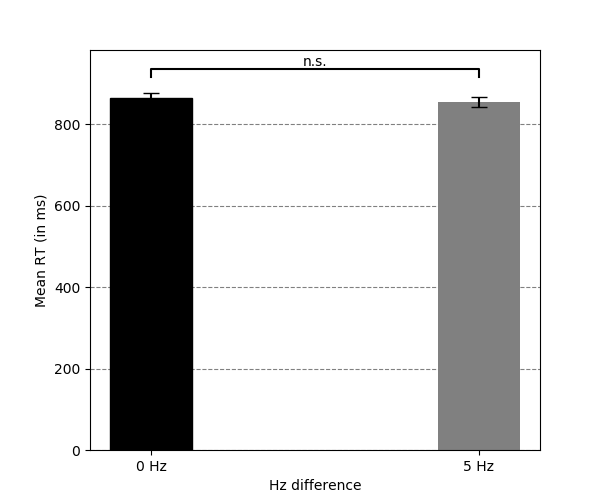
\includegraphics[width=\textwidth]{0Hz_5Hz_bars.png}
    \caption{}
    \label{fig:1a}
  \end{subfigure}\quad
  %
  \begin{subfigure}[h]{0.5\textwidth}
    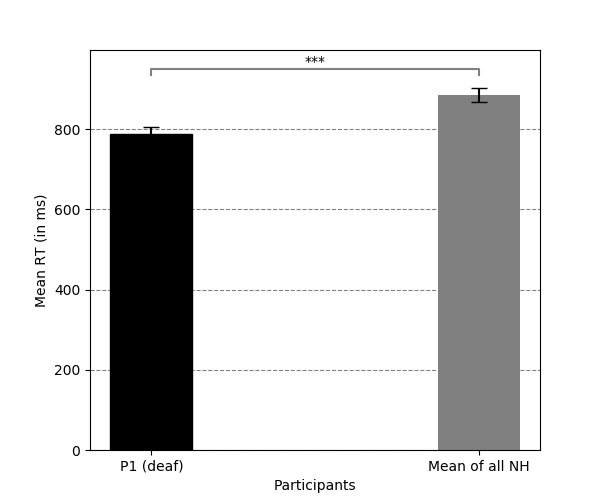
\includegraphics[width=\textwidth]{0Hz_5Hz_deaf_vs_NH.png}
    \caption{}
    \label{fig:1b}
  \end{subfigure}\par
  %
  \centering
  \begin{subfigure}[h]{0.5\textwidth}
    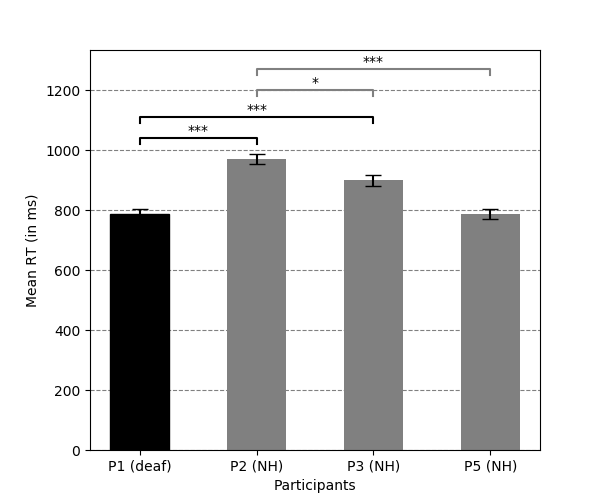
\includegraphics[width=\textwidth]{0Hz_5Hz_all_bars.png}
    \caption{}
    \label{fig:1c}
  \end{subfigure}
\caption{\textit{\footnotesize{Results of the analysis of the 2 (0 Hz difference vs.  5 Hz difference) x 4 (participants) mixed
model. \textbf{(a)}: difference in mean RT between the 0 Hz difference and 5 Hz difference stimulus combinations. \textbf{(b)}: difference in mean RT between the deaf participant and the average normal hearing participant in the sample. \textbf{(c)}: differences between all participants in the sample. \textbf{Annotations}: * for \textit{p} < 0.05; ** for \textit{p} < 0.01; *** for \textit{p} < 0.001; \textit{n.s.} for not significant.}}}
\end{figure*}
%
\begin{figure*}[t!]
  \begin{subfigure}[h]{0.5\textwidth}
    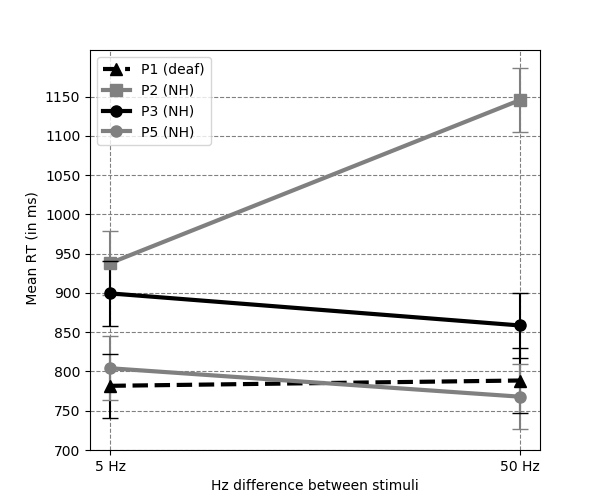
\includegraphics[width=\textwidth]{5Hz_50Hz_interaction.png}
    \caption{}
    \label{fig:2a}
  \end{subfigure}
%
  \begin{subfigure}[h]{0.5\textwidth}
    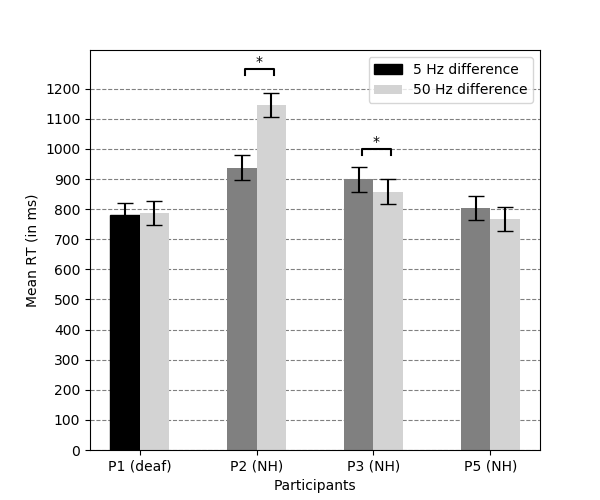
\includegraphics[width=\textwidth]{5Hz_50Hz_all_bar.png}
    \caption{}
    \label{fig:2b}
  \end{subfigure}
\caption{\textit{\footnotesize{Results of the analysis of the 2 (5 Hz difference vs.  50 Hz difference) x 4 (participants) x 472 (trials) mixed
model. \textbf{(a)}: Interaction between the factor stimulus combinations (5 Hz difference vs. 50 Hz difference) and participants. \textbf{(b)}: differences in mean RT between the stimulus combinations per participant. \textbf{Annotations}: * for \textit{p} < 0.05.}}}
\end{figure*}
%
\par The three-way within-subjects ANOVA that was conducted on the second 2 (5 Hz difference vs. 50 Hz difference) x 4 (participants) x 472 (trials) mixed model showed an significant interaction effect between the difference in frequency between stimuli and participant, \textit{F}(3,171) = 4,48, \textit{p} = 0,005, indicating that the effect of difference in frequency between stimuli differed between participants (see Figure 4a). Paired-samples \textit{t}-test were conducted to compare the mean reaction times between trials of 5 Hz difference and 50 Hz difference for each participant separately. The paired samples \textit{t}-test  turned out to be significant for two of the normal-hearing participants. For participant two, there was a significant difference between 5 Hz difference trials (\textit{M} = 938,20, \textit{SD} = 121,14) and 50 Hz difference trials (\textit{M} = 1153,88, \textit{SD} = 784,66); \textit{t}(57) = -2,10, \textit{p} = 0,041, indicating that this participant on average had lower reaction times for the 5 Hz difference trials, compared to 50 Hz difference trials (see Figure 4b). For participant three, there was a significant difference between 5 Hz difference trials (\textit{M} = 899,44, \textit{SD} = 91,5) and 50 Hz difference trials (\textit{M} = 859,7, \textit{SD} = 80,31); \textit{t}(56) = 2,383, \textit{p} = 0,021, indicating that this participant on average had higher reaction times for the 5 Hz difference trials, compared to 50 Hz difference trials (see Figure 4b).
%
\begin{figure*}[t!]
  \begin{subfigure}[h]{0.5\textwidth}
    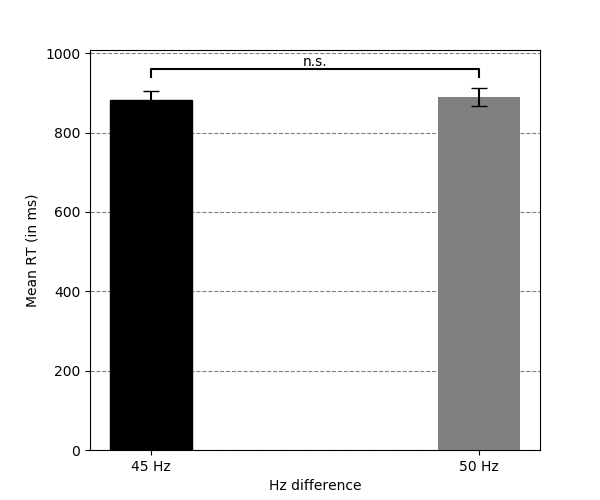
\includegraphics[width=\textwidth]{45Hz_50Hz_bars.png}
    \caption{}
    \label{fig:3a}
  \end{subfigure}\quad
  %
  \begin{subfigure}[h]{0.5\textwidth}
    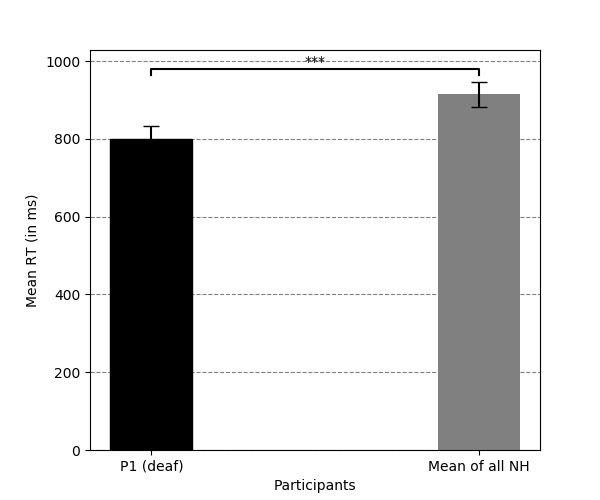
\includegraphics[width=\textwidth]{45Hz_50Hz_deaf_vs_NH.png}
    \caption{}
    \label{fig:3b}
  \end{subfigure}\par
  %
  \centering
  \begin{subfigure}[h]{0.5\textwidth}
    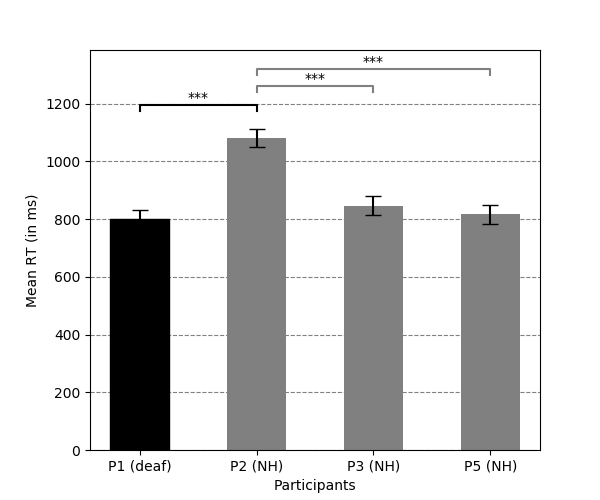
\includegraphics[width=\textwidth]{45Hz_50Hz_all_bars.png}
    \caption{}
    \label{fig:3c}
  \end{subfigure}
\caption{\textit{\footnotesize{Results of the analysis of the 2 (45 Hz difference vs.  50 Hz difference) x 4 (participants) mixed
model. \textbf{(a)}: difference in mean RT between the 45 Hz difference and 50 Hz difference stimulus combinations. \textbf{(b)}: difference in mean RT between the deaf participant and the average normal hearing participant in the sample. \textbf{(c)}: differences in mean RT between all participants in the sample. \textbf{Annotations}: *** for \textit{p} < 0.001; \textit{n.s.} for not significant.}}}
\end{figure*}
%
\par The three-way within-subjects ANOVA that was conducted on the third 2 (45 Hz difference vs. 50 Hz difference) x 4 (participants) x 474 (trials) mixed model showed no significant interaction effect of Hz difference between stimuli and participants, \textit{F}(3,173) = 2,452, \textit{p} = 0,065, indicating that the effect of the difference in frequency between stimuli did not differ between participants. Subsequently, all interaction terms including trial as well as the main effect of trial were removed from the model, leaving a 2 (45 Hz difference vs. 50 Hz difference) x 4 (participants) mixed model. This model was then analyzed using a two-way within-subjects ANOVA (GLM Univariate, IBM SPSS Statistics for Windows, Version 25.0), only including the main effects of the fixed factor difference in frequency between stimuli and random factor participants. 
%
\par Again, the main effect of difference in frequency between stimuli did not reach significance, \textit{F}(1,469) = 0,64, \textit{p} = 0,801, indicating that Hz difference (45 Hz difference vs. 50 Hz difference) did not have an effect on reaction time (see Figure 5a). In contrast to this, the main effect of participant did again reach significance, \textit{F}(3,469) = 17,06, \textit{p} < 0,001, indicating that there was again a significant difference in reaction time between participants. More specifically, there was again a significant difference between the deaf participant (\textit{M} = 801,03, \textit{SE} = 31,73) and the average of all normal-hearing participants (\textit{M} = 914,72, \textit{SE} = 31,82) as was shown by the significance of the Helmert contrast, \textit{Contrast Estimate} = -113,70, \textit{SE} = 36,66, \textit{p} = 0,002). This result pointed towards the conclusion that in the sample, the deaf participant scored significantly lower reaction times than the average of all normal-hearing participants (see Figure 5b). However, exploratory analysis in the form of pairwise comparisons revealed that compared to the deaf participant (\textit{M} = 801,03, \textit{SE} = 31,73), only participant two (\textit{M} = 1080,28, \textit{SE} = 31,60) showed a significant difference in terms of reaction time, \textit{Mean Difference} = -279,25, \textit{SE} = 44,78, \textit{p} < 0,001 (see Figure 5c). Furthermore, this particular participant showed a significant difference not only compared to the deaf participant, but also when compared to the other two normal-hearing participants (\textit{M} = 847, 05, \textit{SE} = 32; \textit{M} = 816,84, \textit{SE} = 31,86), \textit{Mean Difference} = 233,23, \textit{SE} = 45, \textit{p} < 0,001; \textit{Mean Difference} = 263,44, \textit{SE} = 45, \textit{p} < 0,001 (see Figure 5c). This together indicates, that participant two scored exceptionally high reaction times in the sample.
%--------------------------------------------------------------------------------------------
\subsection{Visuo-tactile redundant target paradigm}
The three-way within-subjects ANOVA that was conducted on the first 2 (unisensory vs. multisensory) x 4 (participants) x 3840 (trials) mixed model did not show a significant interaction effect of stimulus configuration and participant, \textit{F}(3,79) = 1,343, \textit{p} = 0,267. This indicated, that the effect of stimulus configuration (i.e. unisensory vs. multisensory) on reaction time did not differ between participants. Subsequently, the factor 'trial' was removed from the model as the main reason for including it in the analysis was to be able to test for the 'stimulus configuration x participants' interaction effect. This left a 2 (unisensory vs. multisensory) x 4 (participants) mixed model. This model was then analyzed using a two-way within-subjects ANOVA (GLM Univariate, IBM SPSS Statistics for Windows, Version 25.0), only including the main effects of fixed factor stimulus configuration and random factor participants. 
%
\par In this model, the main effect of stimulus configuration turned out to be significant, \textit{F}(1,3169) = 662,30, \textit{p} < 0,001, indicating that all participants scored significantly lower reaction times in multisensory trials (\textit{M} = 191,4, \textit{SE} = 1,59) compared to unisensory trials (\textit{M} = 248, \textit{SE} = 1,57) (see Figures 6a and 6b). Furthermore, the main effect of participant also turned out to be significant, \textit{F}(3,3189) = 64,22, \textit{p} < 0,001, indicating that irrespective of stimulus configuration, there was a significant difference between participants in terms of reaction time. As indicated by the significance of the Helmert contrast, \textit{Contrast Estimate} = -27,61, \textit{SE} = 2,56, \textit{p} < 0,001, there was a significant difference in terms of reaction time between the deaf participant (\textit{M} = 199,44, \textit{SE} = 2,21) and the average of all normal-hearing participants (\textit{M} = 227,05, \textit{SE} = 2,25). Again, this result pointed towards the conclusion that in the sample, the deaf participant scored significantly lower reaction times than the average of all normal-hearing participants (see Figure 6a and 6c). Exploratory analysis in the form of individual pairwise comparisons between the deaf participant and normal-hearing participants supported this interpretation as they all turned out to be significant (all \textit{p} < 0,001) (see Figure 6d). Even though this time none of the normal-hearing participants scored exceptionally high reaction times compared to the others, participant two (\textit{M} = 219,44, \textit{SE} = 2,22) and participant three (\textit{M} = 219,42, \textit{SE} = 2,35) scored almost identical mean reaction times, \textit{Mean Difference} = 0,019, \textit{SE} = 3,24, \textit{p} = 1,00 (see Figure 6d).
%
\begin{figure*}[h!]
        \centering
        \begin{subfigure}[b]{0.475\textwidth}
            \centering
            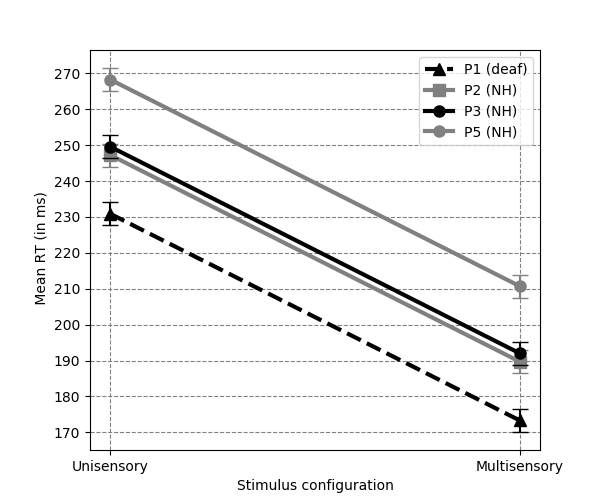
\includegraphics[width=\textwidth]{Uni_Multi_lines.png}
            \caption[]%
            {{\small}}    
            \label{fig:4a}
        \end{subfigure}
        \hfill
        \begin{subfigure}[b]{0.475\textwidth}  
            \centering 
            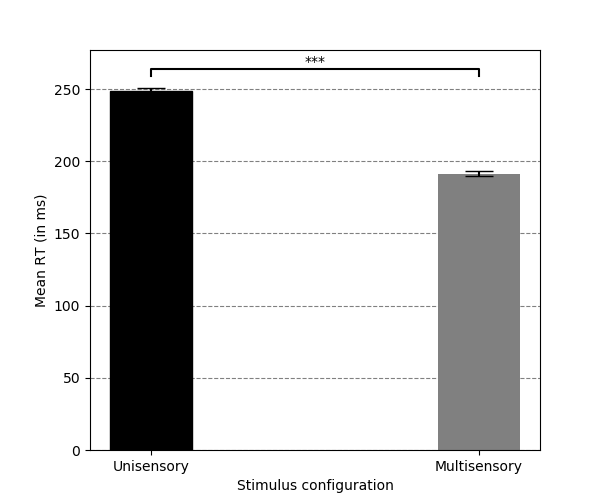
\includegraphics[width=\textwidth]{Uni_Multi_bar.png}
            \caption[]%
            {{\small}}    
            \label{fig:4b}
        \end{subfigure}
        \vskip\baselineskip
        \begin{subfigure}[b]{0.475\textwidth}   
            \centering 
            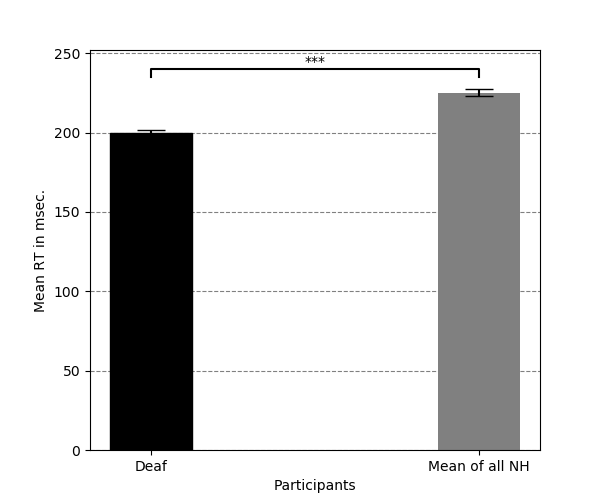
\includegraphics[width=\textwidth]{Uni_Multi_deaf_meanNH_bar.png}
            \caption[]%
            {{\small}}    
            \label{fig:4c}
        \end{subfigure}
        \quad
        \begin{subfigure}[b]{0.475\textwidth}   
            \centering 
            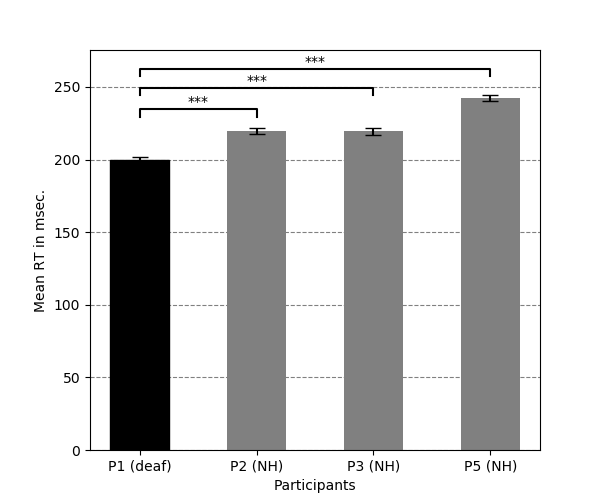
\includegraphics[width=\textwidth]{Uni_Multi_all_bar.png}
            \caption[]%
            {{\small}}    
            \label{fig:4d}
        \end{subfigure}
        \caption[]%
        {\textit{\footnotesize{Results of the analysis of the 2 (unisensory vs. multisensory) x 4 (participants) mixed
model. \textbf{(a)}: difference in mean RT between stimulus configurations (unisensory vs. multisensory) per participant. \textbf{(b)}: difference in mean RT between unisensory and multisensory stimulus configurations. \textbf{(c)}: difference in mean RT between the deaf participant and the average normal hearing participant in the sample. \textbf{(d)}: differences in mean RT between all participants in the sample. \textbf{Annotations}: *** for \textit{p} < 0.001.}}} 
        \label{fig:mean and std of nets}
\end{figure*}
%
\par The three-way within-subjects ANOVA that was conducted on the second 2 (spatially aligned vs. non-spatially aligned ) x 4 (participants) x 3840 (trials) mixed model did not show a significant interaction effect of stimulus configuration and participant, \textit{F}(3,88) = 0,939, \textit{p} = 0,427, indicating that the effect of stimulus configuration (i.e. spatially aligned vs. non-spatially aligned) did not differ between participants. Therefore, all interaction terms including trial as well as the main effect of trial were removed from the model, leaving a 2 (spatially aligned vs. non-spatially aligned) x 4 (participants) mixed model. This model was then analyzed using a two-way within-subjects ANOVA (GLM Univariate, IBM SPSS Statistics for Windows, Version 25.0), only including the main effects of fixed factor stimulus configuration and random factor participants. 
%
\par The main effect of stimulus configuration did not reach significance, \textit{F}(1,1568) = 0,000, \textit{p} = 0,991, indicating that there was generally no difference in terms of reaction times between trials of spatially aligned multisensory stimuli (\textit{M} = 191,32, \textit{SE} = 2,1) and trials of non-spatially aligned multisensory stimuli (\textit{M}= 191,35, \textit{SE}, 2,18)(see Figure 7). The main effect of participant turned out to be significant, \textit{F}(3,1568) = 45,34, \textit{p} < 0,001, again indicating that irrespective of stimulus configuration, there was a significant difference between participants in terms of reaction time. Again, the Helmert contrast was significant, \textit{Contrast Estimate} = -31,15, \textit{SE} = 3,45, \textit{p} < 0,001, indicating that the deaf participant (\textit{M} = 168, \textit{SE} = 3) overall scored significantly lower reaction times compared to the average of all normal-hearing participant (\textit{M} = 199,12, \textit{SE} = 3,03). This result again showed that on average, the deaf participant scored lower reaction times for multisensory stimulus configurations compared to normal-hearing controls (see Figures 4a and 4c).
%
\begin{figure*}[t!]
    \centering
    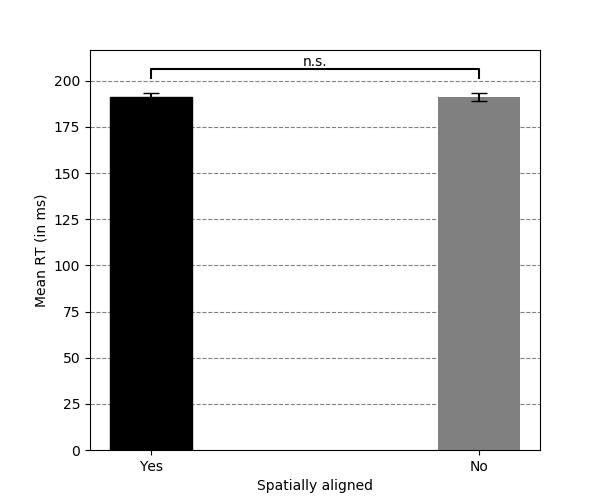
\includegraphics[width=0.7\textwidth]{SAlign_Yes_No.png}
    \caption{\textit{\footnotesize{Difference in mean RT between spatially aligned and non-spatially aligned multisensory stimulus configurations. \textbf{Annotations}: \textit{n.s.} for not significant.}}}
    \label{fig:5}
\end{figure*}
%
\begin{figure*}[t!]
        \centering
        \begin{subfigure}[b]{0.475\textwidth}
            \centering
            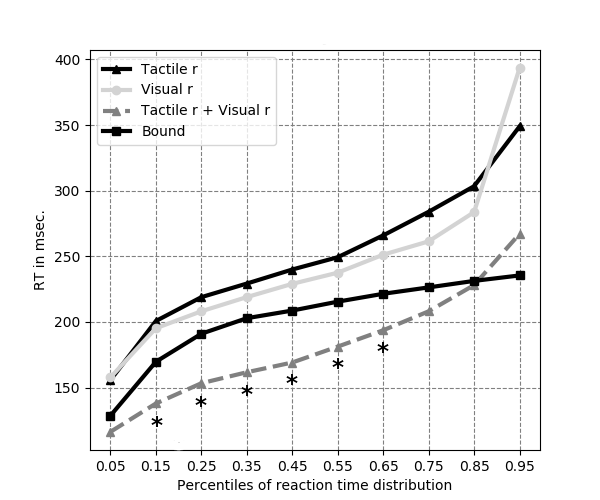
\includegraphics[width=\textwidth]{RMITest_VrTr_lines.png}
            \caption[]%
            {{\small}}    
            \label{fig:6a}
        \end{subfigure}
        \hfill
        \begin{subfigure}[b]{0.475\textwidth}  
            \centering 
            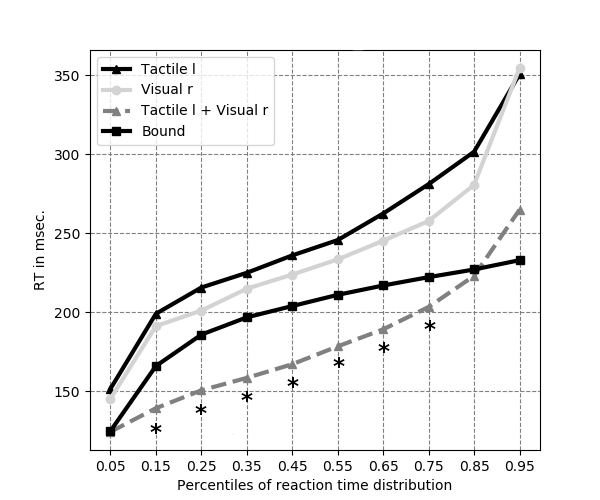
\includegraphics[width=\textwidth]{RMITest_VrTl_lines.png}
            \caption[]%
            {{\small}}    
            \label{fig:6b}
        \end{subfigure}
        \vskip\baselineskip
        \begin{subfigure}[b]{0.475\textwidth}   
            \centering 
            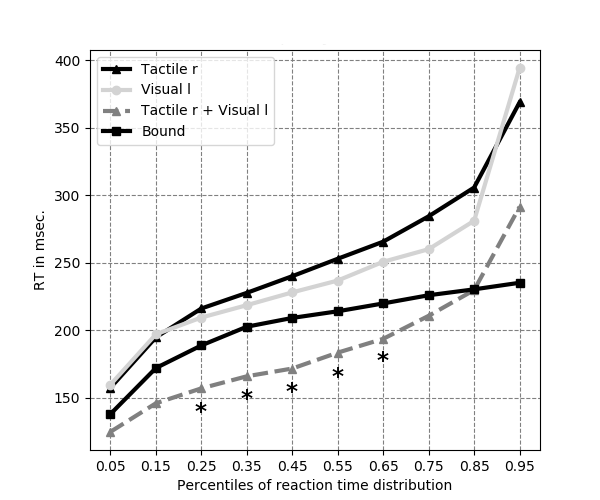
\includegraphics[width=\textwidth]{RMITest_VlTr_lines.png}
            \caption[]%
            {{\small}}    
            \label{fig:6c}
        \end{subfigure}
        \quad
        \begin{subfigure}[b]{0.475\textwidth}   
            \centering 
            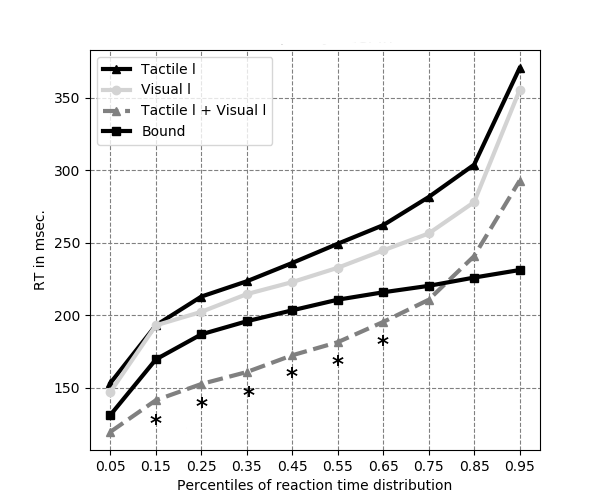
\includegraphics[width=\textwidth]{RMITest_VlTl_lines.png}
            \caption[]%
            {{\small}}    
            \label{fig:6d}
        \end{subfigure}
        \caption[]%
        {\textit{\footnotesize{Results of the analysis of race model inequality using RMITest software \parencite{ulrich_testing_2007} across all participants in the sample. Lines represent cumulative density functions of the reaction time distributions of respective stimulus configurations."Bound" values were calculated based on the cumulative density distributions of unisensory stimulus configurations and represent the upper boundaries for predictions of multisensory gain based on race models \parencite{miller_divided_1982,ulrich_testing_2007}. Observations below "bound" values indicate voilations of race model predictions. \textbf{(a)}: race model violations for the spatially aligned tactile right/visual right multisensory stimulus configuration. \textbf{(b)}: race model violations for the non-spatially aligned tactile left/visual right multisensory stimulus configuration. \textbf{(c)}: race model violations for the non-spatially aligned tactile right/visual left multisensory stimulus configuration. \textbf{(d)}: race model violations for the spatially aligned tactile left/visual left multisensory stimulus configuration. \textbf{Annotations}: * for \textit{p} < 0.05.}}} 
        \label{fig:6}
\end{figure*}
%
\par The analysis of race model inequality using RMITest software \parencite{ulrich_testing_2007} indicated, that the observed redundancy gain for multisensory stimulus configurations significantly exceeded race model predictions based on statistical facilitation for the fastest percentiles of reaction times (all \textit{p} < 0.05)\parencite{miller_divided_1982, ulrich_testing_2007}(see Figure 8 a-d). Furthermore, this was the case irrespective of spatial alignment of multisensory stimuli (see Figure 8 a-d). We therefore attributed the observed redundancy gain to a coactivation process underlying multisensory integration \parencite{miller_divided_1982,miller_timecourse_1986}.
%----------------------------------------------------------------------------
\section{Discussion}
The aim of the present study was to add to the understanding of changes in sensory processing in response to the deficit or loss of one sensory modality. Specifically, the present study investigated the difference in tactile acuity and visuotactile multisensory integration between a congenitally deaf participant and a control group of three normal-hearing participants. To investigate tactile acuity, participants performed a two-interval forced-choice vibrotactile frequency discrimination task \parencite{alary_tactile_2009}. To investigate multisensory integration, participants preformed a simple reaction time visuo-tactile redundant target paradigm \parencite{girard_multisensory_2011}. In addition, it was investigated whether the observed reduction in reaction time for multiensory stimuli compared to unisensory stimuli (i.e. redundancy gain) exceeded predictions based on race models and could therefore be be attributed to a coactivation process \parencite{miller_divided_1982,ulrich_testing_2007}.
%----------------------------------------------------------------------------
\par For the vibrotactile frequency discrimination task, the comparison between the 125 Hz and 125 Hz stimulus combination (0 Hz difference) and the 125 Hz and 130 Hz stimulus combination (5 Hz difference) indicated, that there was no difference in effect on reaction time between the two stimulus combinations containing the two smallest differences in frequency. Furthermore, the results indicated that for stimulus combinations of no or low differences in frequency the deaf participant was generally faster in perceiving the stimuli and making a judgment about their equivalence compared to the average normal-hearing participant in the sample. However, it is important to note that the deaf participant scored significantly lower reaction times only compared to two out of the three normal-hearing participants (participant two and participant five) in the sample. In addition, participant two also scored significantly higher reaction times than the the other two normal-hearing participants. Thus, it must be assumed that the extraordinarily high reaction times of participant two have led to the overall significant difference between the deaf and the average normal hearing participant in the sample. 
%
\par For the comparison between the 125 Hz and 130 Hz stimulus combination (5 Hz difference) and the 125 Hz and 175 Hz stimulus combination (50 Hz difference), only two of the normal hearing participants showed a significant difference in reaction time of which only one was in the expected direction. Participant two showed a much higher reaction time in 50 Hz difference trials than compared to the 5 Hz difference trials. This was very unusual as the 50 Hz difference is the maximum difference between stimuli and was therefore thought to be the most unambiguous difference that should lead to very fast reaction times. All other participants in the sample showed either equal reaction times as compared to the 5 Hz difference or even lower ones, as was observed for participant three (and participant four, although not significant). Participant two had already shown extraordinarily  high reaction times compared to the rest of the sample in the first analysis comparing the 0 Hz difference and the 5 Hz difference combinations (see paragraph above). Therefore, the unusual pattern of reaction times observed in this analysis can most likely again be attributed to a poor performance in the task by participant two.
%
\par The comparison between the 125 Hz and 170 Hz stimulus combination (45 Hz difference) and the 125 Hz and 175 Hz stimulus combination (50 Hz difference) yielded a similar picture as the first analysis (0 Hz difference vs. 5 Hz difference). Even though overall, there was no difference in effect on reaction time between the two stimulus combinations containing the two largest differences in frequency, the deaf participant again seemed to be faster in perceiving the stimuli and making a judgment about their equivalence than the average normal-hearing participant in the sample. However, upon closer investigation it again became clear that this difference was most likely caused by the particularly poor performance by participant two, who was the only normal-hearing participant in the sample to show a significant difference to the deaf participant.
%
\par Taken together, the results of our analysis of reaction times obtained in the vibrotactile frequency discrimination task do not support the hypothesis that the deaf participant shows enhanced tactile acuity for vibrotactile stimuli compared to normal-hearing participants. Even though differences between the deaf subject and the average normal-hearing participant did emerge in our sample, they appear to be biased by the particularly poor performance of one of the normal-hearing participants. Our findings are therefore not in line with previous research that reported enhanced tactile acuity for vibrotactile stimuli in deaf participants as compared to normal-hearing participants \parencite{levanen_feeling_2001,schiff_deaf_1972}. However, our findings are also not in line with previous research that found lower tactile acuity in deaf participants as compared to normal-hearing participants \parencite{frenzel_genetic_2012,moshourab_congenital_2017}. Instead, our findings are more in line with the results by \cite{moallem_measures_2010} who reported no difference in detection thresholds for vibratory tactile stimuli between groups of deaf and normal-hearing participants.
%---------------------------------------------------------------------------------------
\par Concerning the results of the visuo-tactile redundant target paradigm, all participants in our sample showed significant redundancy gains (i.e. shorter reaction times) for multisensory stimulus configurations. This observation is in line with previous findings \parencite{diederich_bimodal_2004,hershenson_reaction_1962,miller_divided_1982}. Furthermore, the deaf participant in our sample was faster in reacting to both unisensory and multisensory stimulus configurations compared to the average normal-hearing participant. This time, this conclusion seemed not to be biased by the particularly poor performance of one of the normal-hearing participants. The observation that in our sample, the deaf participant was faster in responding to unisensory stimuli compared to normal-hearing controls was interesting. Unisensory stimuli were either visual or vibrotactile. Hence, based on the results of the vibrotactile frequency discrimination task which indicated no enhanced tactile acuity of the deaf participant, it could be assumed that the overall faster reaction to unisensory stimuli was due to faster reactions to visual stimuli. This is for now a mere speculation, as it has not specifically been tested for in the present study. Nevertheless, it would be in line with previous research that indicated enhanced visual processing in the deaf \parencite{proksch_changes_2002}. Additionally, it must be noted that the two tasks used two different reaction time paradigms. While the vibrotactile frequency discrimination task was a choice reaction time task, the visuotactile redundant target paradigm was a simple reaction time task. This difference might also account for the different results in terms of performance of the deaf participant in the sample. 
%---------------------------------------------------------------------------------------
\par The most interesting finding was, that in our sample the deaf participant profited just as much from multisensory stimulus configurations in terms of multisensory gain (i.e. reduction in reaction time) as did the normal-hearing controls. This indicates, that the deaf participant in our sample showed no deficit in visuotactile multisensory integration compared to normal-hearing controls. This observation is inconsistent with previous research that mostly indicated deficits in multisensory integration following sensory loss or deficit \parencite{champoux_early-_2011,occelli_audiotactile_2012,hotting_hearing_2004,landry_temporary_2013}. Particularly, our results are inconsistent with results by Hauthal and colleagues (2015), who demonstrated a significantly higher redundancy gain for normal-hearing participants as compared to deaf participants, using a visuo-tactile redundant target paradigm similar to the one that was used in the present study. 
\par Lastly, we replicated findings by Girard, Collingnon and Lepore (2011), showing that across all participants in our sample the observed redundancy gains for multisensory stimuli clearly violated race model predictions. We therefore attribute the observed multisensory enhancement to a coactivation process, rather than a parallel activation process underlying multisensory integration \parencite{miller_divided_1982,miller_timecourse_1986,ulrich_testing_2007}. Furthermore, similar to the findings by Girard, Collingnon and Lepore (2011) the spatial configuration of stimuli did not have an influence on multisensory gain and race model violation. 
%
\par A major limitation of the present study were the low and unequal sample sizes of only one deaf participant and three normal-hearing participants. As was mentioned earlier, this limited the implications of our results to the sample and no inferences could be made on the population level (see section 2.3 Data analysis). With the low and unequal sample size came the possibility that one influential case could easily lead to a significant difference between the deaf participant and normal-hearing participants, as has been observed for the vibrotactile frequency discrimination task. Furthermore, given the fact that our results cannot be generalized to the population level, they are only to a limited extent comparable to the results of other studies that could make such inferences.
%
\par The fact that the analysis for the vibrotactile frequency discrimination task comprised only the comparison of three selected pairs of stimulus combinations (0 Hz difference vs. 5 Hz difference; 5 Hz difference vs. 50 Hz difference; 45 Hz difference vs. 50 Hz difference) can be seen as another limitation of the present study. The selection of these three pairs of stimulus combinations was based on the intention to keep the analysis concise, while still being able to draw conclusions about differences between the deaf participant and normal-hearing participants. However, it could be the case that a more extensive analysis including more comparisons between stimulus combinations would have yielded somewhat different results. Another limitation of our study is that accuracy scores of participants were not taken into account in the analysis. It could therefore be assumed, that clearer differences between the deaf and normal-hearing participants would have emerged if not only reaction time would have been investigated. 
%----------------------------------------------------------------------------
\section{Conclusion}
Our study does not provide evidence for enhanced tactile acuity for vibrotactile stimuli in deaf participants, based on the available sample. Instead, the deaf participant in our sample showed levels of tactile acuity similar to those of normal-hearing controls, based on performance in a vibrotactile frequency discrimination task. Furthermore, the deaf participant in our sample showed visuo-tactile multisensory integration in the same way as did normal-hearing controls in a visuo-tactile multisensory integration task. Lastly, redundancy gains (i.e. shorter reaction time) for multisensory stimuli that were observed for participants in our sample significantly exceeded race model predictions. They were therefore attributed to a coactivation process underlying multisensory integration. Due to a very limited sample size, these findings cannot be generalized to the population.
%----------------------------------------------------------------------------
\section{Acknowledgements}
I would like to express my sincere gratitude to Franco Lepore and Emma Campbell for allowing me to join their research project and for their support and guidance during my exchange semester at the Université de Montréal. In addition, I would like to thank Nick Broers for his support and advice. Lastly, I would like to thank Arie van der Lugt for organizing the MaRBLe programme for students at the Faculty of Psychology and Neuroscience.
\printbibliography 
\end{document}